%license:BSD-3-Clause
%copyright-holders:Michele Maione
%============================================================
%
%	Piattaforma di cloud gaming per giochi arcade
%
%============================================================
\chapter{Implementazione}
%In questa sezione si spiega come è stato affrontato il problema concettualmente, la soluzione logica che ne è seguita senza la documentazione.
%Si mostra il progetto dell’architettura del sistema con i vari moduli.
In questo capitolo verranno descritte le cinque fasi aggiuntive del cloud gaming e la loro implementazione in C++ come nuovi moduli del MAME: la cattura audio-video, la codifica, la trasmissione, la decodifica e la gestione dell'input utente.




\section{Cattura}
Nel paradigma del cloud gaming per cattura si intende la fase in cui l'output audio-visivo del videogioco viene messo da parte per essere poi inviato al codificatore. Nei prossimi due paragrafi vedremo i metodi di cattura per la parte video e per quella audio.


\subsection{Video}
Per la cattura video esistono tre metodi di cattura: l'hook di funzioni della libreria multimediale, l'utilizzo delle API per il framebuffer virtuale e l'uso di schede video con funzionalità di codifica incorporata.

L'hook di funzione è una tecnica di programmazione con la quale si sostituisce il comportamento di una funzione di un programma o di una libreria già compilata. Questa operazione su una libreria multimediale consiste nel modificare il normale funzionamento della procedura che invia il framebuffer della scheda video all'uscita. Ad esempio per le librerie multimediali più usate le funzioni da catturare sono: \verb|SDL_RenderPresent| per SDL, \verb|Present| per DirectX e \verb|SwapBuffer| per OpenGL \parencite{GamingAnywhere}. Questo metodo è stato usato ad esempio da OnLive, Gaikai e Vortex. Un esempio di codice per l'hook di funzioni per SDL è mostrato nel Lis. \ref{lst:hookCode}.

\begin{lstlisting}[caption=Codice di hook per la libreria SDL, label={lst:hookCode}]
	HOOK_TRACE_INFO hHook = { NULL };
	
	HMODULE lib_handle = LoadLibrary("SDL2.dll");

	FARPROC old_SDL_RenderPresent =	GetProcAddress(
		lib_handle, "SDL_RenderPresent");

	NTSTATUS result = LhInstallHook(
		old_SDL_RenderPresent, my_SDL_RenderPresent,
		NULL, &hHook);
\end{lstlisting}

Il framebuffer virtuale è una funzionalità offerta dalle API di sistema per accedere all'attuale framebuffer presente nella scheda video. Il loro utilizzo principale è per il remote desktop, ma alcune piattaforme come "GamingAnywhere" \parencite{GamingAnywhere} e "Parsec"\footnote{Parsec è un servizio di desktop remoto basato su Windows offerto dalla omonima società.} \parencite{TheTechnologyBehindALowLatencyCloudGamingService} utilizzano questa funzionalità per la cattura video, il primo per la piattaforma di cloud gaming, il secondo per offrire un computer virtuale. Alcuni esempi nei moderni sistemi operativi sono: "X virtual framebuffer" su Linux X11 \parencite{XVFB}, "Desktop Duplication API" su Windows \parencite{DesktopDuplicationAPI} e \verb|CGDisplayStream| della libreria "Quartz Display Services" su macOS.

La prima società che modificò una scheda video adattandola per il cloud gaming fu Sony che incluse un chip di codifica sulle GPU Nvidia ed AMD (rispettivamente per il rendering PS3 e PS4) \parencite{PlayStation_Now_Chip}. Altre piattaforme di cloud gaming che usano schede video con funzionalità di encoding incluse sono "Nvidia GeForce Now" su schede Nvidia \parencite{GeForce_Now}, "Microsoft XBox Cloud Gaming" su schede AMD \parencite{xCloudBlade}, "Google Stadia" su AMD \parencite{Google_Stadia_Server} e "Amazon Luna" su Nvidia \parencite{Amazon_Luna_GPU}. La lista delle aziende che creano schede video con questa funzionalità è riportata in Tab. \ref{table:VideoCardEncodingFeature} \parencite{NVIDIAVideoCodecSDK} \parencite{GCNArchitecture} \parencite{IntelQuickSyncVideo} \parencite{Hexagon_DSP_SDK}.

\begin{table}[H]
	\centering
	\begin{tabular}{||c c c||} 
		\hline
		Produttore & Funzionalità & Codec supportati \\
		\hline\hline
		Nvidia & NVENC & AVC, HEVC \\
		\hline
		AMD & Video Core Next & AVC, HEVC \\
		\hline
		Intel & Quick Sync Video & MPEG-2, AVC, HEVC, VP8, VP9 \\
		\hline
		Qualcomm & Hexagon & H.263, MPEG-4, AVC, HEVC, VP8, VP9 \\
		\hline
	\end{tabular}

	\caption{Schede video con funzionalità di codifica video}
	\label{table:VideoCardEncodingFeature}
\end{table}

Poiché del progetto MAME sono disponibili i sorgenti in questo progetto ho scelto di modificare il comportamento normale del programma. Come mostrato in Fig. \ref{fig:class_renderingSDLFull_Streaming}, sono state aggiunte alla classe \verb|renderer_sdl2| le due funzioni (\verb|init_streaming_render| e \verb|free_streaming_render|) per allocare e deallocare le strutture dati per la cattura. Come mostrato nel Lis. \ref{lst:init_streaming_render_init} le funzioni della libreria SDL che sono state aggiunte al codice sono:

\begin{itemize}
	\item CreateRGBSurfaceWithFormat: crea una superficie RGB specificando il formato pixel da utilizzare;	
	\item CreateSoftwareRenderer: crea un contesto di rendering 2D per una superficie;
	\item RWFromMem: prepara un buffer di memoria di lettura-scrittura da utilizzare con la struttura dati RWops (read-write opaque pointer structure).	
\end{itemize}

\begin{lstlisting}[caption=Codice aggiunto per la cattura video: inizializzazione, label={lst:init_streaming_render_init}]
	sdl_buffer_bytes_length = w * h * 4; // RGBA = 4 bytes
	sdl_buffer_bytes = new char[sdl_buffer_bytes_length];

	sdl_surface = SDL_CreateRGBSurfaceWithFormat(
		0, w, h, 32, SDL_PIXELFORMAT_RGBA32);
	
		sdl_renderer = SDL_CreateSoftwareRenderer(sdl_surface);
	
	sdl_buffer = SDL_RWFromMem(
		sdl_buffer_bytes, sdl_buffer_bytes_length);
\end{lstlisting}

Nel Lis. \ref{lst:init_streaming_render_draw} è mostrato il codice che è stato inserito per inviare alla classe statica che gestisce lo streaming (\verb|streaming_server|) il frame da inviare al giocatore (che verrà codificato prima dell'invio). Poiché l'attuale contesto di rendering (\verb|sdl_renderer|) è creato su una superfice RGB (\verb|sdl_surface|) quando il contesto di rendering viene aggiornato con il framebuffer corrente (tramite \verb|SDL_RenderPresent|) è la superfice a ricevere il frame attuale.

\begin{lstlisting}[caption=Codice aggiunto per la cattura video: disegno, label={lst:init_streaming_render_draw}]
	SDL_RenderPresent(sdl_renderer);

	streaming_server::instance()
		.send_video_frame(sdl_surface->pixels);

	// riposizionamento all'inizio del buffer	
	SDL_RWseek(sdl_buffer, 0, RW_SEEK_SET);
\end{lstlisting}

\begin{figure}[H]
	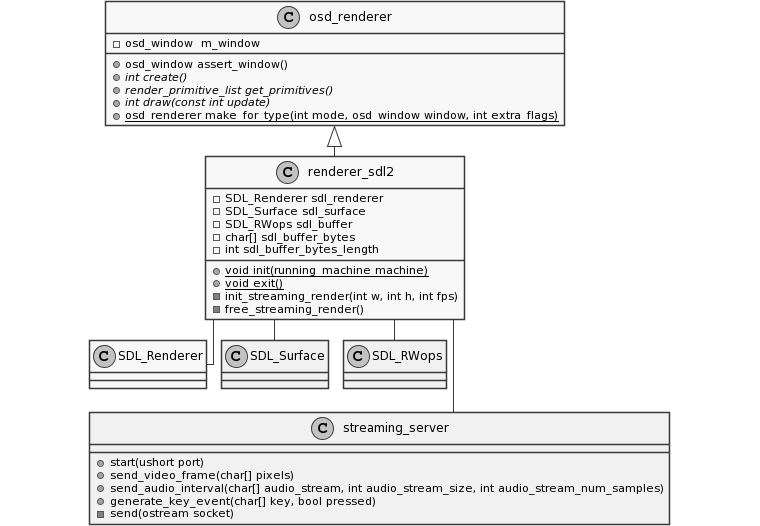
\includegraphics[width=\linewidth]{immagini/class_renderingSDLFull_Streaming}
	\caption{Diagramma delle classi relative alla cattura video}
	\label{fig:class_renderingSDLFull_Streaming}
\end{figure}

I listati precedenti sono stati estrapolati dal Lis. \ref{lst:draw13} disponibile in appendice \ref{chap:Listato}.



\subsection{Audio} \label{Cattura_Audio}
Come per la cattura video si può ricorrere all'hook di funzioni della libreria multimediale o alle API del sistema operativo per la gestione audio \parencite{GamingAnywhere}. In quest'ultimo caso abbiamo "Windows Audio Session API" per Windows \parencite{WASAPI}, "Advanced Linux Sound Architecture" per Linux \parencite{ALSA} e "Core Audio" per macOS \parencite{Core_Audio_api}.

Come nel caso della cattura video ho scelto di modificare il sorgente del programma. Come mostrato in Fig. \ref{fig:class_mixingSDL_streaming} la classe \verb|sound_sdl| implementa la funzione di callback necessaria per utilizzare il missaggio audio di SDL, di cui abbiamo parlato nel paragrafo \ref{chap:Missaggio_audio}. All'interno di questa funzione, tramite la funzione \verb|send_audio_interval|, è stato inviato alla classe che si occupa di gestire il server di streaming (\verb|streaming_server|) il buffer sonoro (\verb|stream|) e la sua dimensione (\verb|len|). La modifica apportata è mostrata nel Lis. \ref{lst:sdl_sound_callback}.

\begin{lstlisting}[caption=Codice aggiunto per la cattura audio, label={lst:sdl_sound_callback}]
	streaming_server::instance().send_audio_interval(
			stream, len, 512); // 512 campioni audio (per canale)

	memset(stream, 0, len); // svuota buffer sonoro
\end{lstlisting}


\begin{figure}[H]
	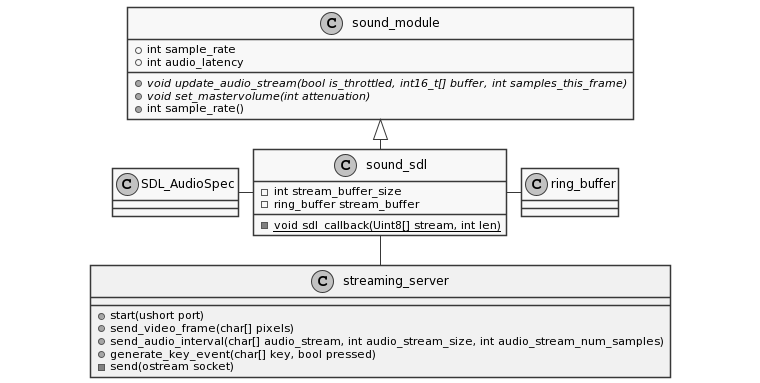
\includegraphics[width=\linewidth]{immagini/class_mixingSDL_streaming}
	\caption{Diagramma delle classi relative alla cattura audio}
	\label{fig:class_mixingSDL_streaming}
\end{figure}

I listati precedenti sono stati estrapolati dal Lis. \ref{lst:sdl_sound} disponibile in appendice \ref{chap:Listato}.

\section{Codifica}
Lorem ipsum dolor sit amet, consectetur adipiscing elit, sed do eiusmod tempor incididunt ut labore et dolore magna aliqua. Ut enim ad minim veniam, quis nostrud exercitation ullamco laboris nisi ut aliquip ex ea commodo consequat. Duis aute irure dolor in reprehenderit in voluptate velit esse cillum dolore eu fugiat nulla pariatur. Excepteur sint occaecat cupidatat non proident, sunt in culpa qui officia deserunt mollit anim id est laborum.

\subsection{MPEG}
Lorem ipsum dolor sit amet, consectetur adipiscing elit, sed do eiusmod tempor incididunt ut labore et dolore magna aliqua. Ut enim ad minim veniam, quis nostrud exercitation ullamco laboris nisi ut aliquip ex ea commodo consequat. Duis aute irure dolor in reprehenderit in voluptate velit esse cillum dolore eu fugiat nulla pariatur. Excepteur sint occaecat cupidatat non proident, sunt in culpa qui officia deserunt mollit anim id est laborum.

\subsubsection{Compression}
Lorem ipsum dolor sit amet, consectetur adipiscing elit, sed do eiusmod tempor incididunt ut labore et dolore magna aliqua. Ut enim ad minim veniam, quis nostrud exercitation ullamco laboris nisi ut aliquip ex ea commodo consequat. Duis aute irure dolor in reprehenderit in voluptate velit esse cillum dolore eu fugiat nulla pariatur. Excepteur sint occaecat cupidatat non proident, sunt in culpa qui officia deserunt mollit anim id est laborum.

\subsubsection{Video}
Lorem ipsum dolor sit amet, consectetur adipiscing elit, sed do eiusmod tempor incididunt ut labore et dolore magna aliqua. Ut enim ad minim veniam, quis nostrud exercitation ullamco laboris nisi ut aliquip ex ea commodo consequat. Duis aute irure dolor in reprehenderit in voluptate velit esse cillum dolore eu fugiat nulla pariatur. Excepteur sint occaecat cupidatat non proident, sunt in culpa qui officia deserunt mollit anim id est laborum.

\subsubsection{Audio}
Lorem ipsum dolor sit amet, consectetur adipiscing elit, sed do eiusmod tempor incididunt ut labore et dolore magna aliqua. Ut enim ad minim veniam, quis nostrud exercitation ullamco laboris nisi ut aliquip ex ea commodo consequat. Duis aute irure dolor in reprehenderit in voluptate velit esse cillum dolore eu fugiat nulla pariatur. Excepteur sint occaecat cupidatat non proident, sunt in culpa qui officia deserunt mollit anim id est laborum.

\subsubsection{Trasmission}
Lorem ipsum dolor sit amet, consectetur adipiscing elit, sed do eiusmod tempor incididunt ut labore et dolore magna aliqua. Ut enim ad minim veniam, quis nostrud exercitation ullamco laboris nisi ut aliquip ex ea commodo consequat. Duis aute irure dolor in reprehenderit in voluptate velit esse cillum dolore eu fugiat nulla pariatur. Excepteur sint occaecat cupidatat non proident, sunt in culpa qui officia deserunt mollit anim id est laborum.

\subsection{FFmpeg}
Lorem ipsum dolor sit amet, consectetur adipiscing elit, sed do eiusmod tempor incididunt ut labore et dolore magna aliqua. Ut enim ad minim veniam, quis nostrud exercitation ullamco laboris nisi ut aliquip ex ea commodo consequat. Duis aute irure dolor in reprehenderit in voluptate velit esse cillum dolore eu fugiat nulla pariatur. Excepteur sint occaecat cupidatat non proident, sunt in culpa qui officia deserunt mollit anim id est laborum \parencite{FFmpeg_Documentation}.

\subsubsection{Libs.}
Lorem ipsum dolor sit amet, consectetur adipiscing elit, sed do eiusmod tempor incididunt ut labore et dolore magna aliqua. Ut enim ad minim veniam, quis nostrud exercitation ullamco laboris nisi ut aliquip ex ea commodo consequat. Duis aute irure dolor in reprehenderit in voluptate velit esse cillum dolore eu fugiat nulla pariatur. Excepteur sint occaecat cupidatat non proident, sunt in culpa qui officia deserunt mollit anim id est laborum.




\section{Trasmissione}
Lorem ipsum dolor sit amet, consectetur adipiscing elit, sed do eiusmod tempor incididunt ut labore et dolore magna aliqua. Ut enim ad minim veniam, quis nostrud exercitation ullamco laboris nisi ut aliquip ex ea commodo consequat. Duis aute irure dolor in reprehenderit in voluptate velit esse cillum dolore eu fugiat nulla pariatur. Excepteur sint occaecat cupidatat non proident, sunt in culpa qui officia deserunt mollit anim id est laborum.

\subsection{Web APIs}
Le API Web sono un insieme di API e interfacce che comprendono la potente capacità di creazione di script del Web. A seguire quelli utilizzati in questo progetto \parencite{Web_APIs}.

\subsubsection{WebSocket}
WebSocket è un protocollo di comunicazione del computer che fornisce canali di comunicazione full-duplex su una singola connessione TCP. È compatibile con HTTP perché l'handshake WebSocket utilizza l'intestazione di aggiornamento HTTP per passare dal protocollo HTTP al protocollo WebSocket. È supportato nativamente da tutti i browser e il suo utilizzo è simile ai normali socket sia sul lato client che su quello server. Per questi motivi è il protocollo di comunicazione generico più utilizzato sul web \parencite{WebSocket_Web_APIs}.




\section{Decodifica}
Lorem ipsum dolor sit amet, consectetur adipiscing elit, sed do eiusmod tempor incididunt ut labore et dolore magna aliqua. Ut enim ad minim veniam, quis nostrud exercitation ullamco laboris nisi ut aliquip ex ea commodo consequat. Duis aute irure dolor in reprehenderit in voluptate velit esse cillum dolore eu fugiat nulla pariatur. Excepteur sint occaecat cupidatat non proident, sunt in culpa qui officia deserunt mollit anim id est laborum.

\subsection{Web APIs}
Le API Web sono un insieme di API e interfacce che comprendono la potente capacità di creazione di script del Web. A seguire quelli utilizzati in questo progetto \parencite{Web_APIs}.

\subsubsection{Canvas API}
L'API Canvas fornisce un mezzo per disegnare grafica tramite JavaScript, si concentra principalmente sulla grafica 2D ma quando viene utilizzata dall'API WebGL può disegnare grafica 2D e 3D con accelerazione hardware. È completamente supportato da tutti i browser \parencite{Canvas_API}.

\subsubsection{WebGL API}
WebGL è un'API JavaScript, progettata e gestita dal gruppo no-profit Khronos, per il rendering di grafica 2D e 3D che consente l'utilizzo accelerato dalla GPU della fisica e dell'elaborazione e degli effetti delle immagini. WebGL 1.0 è supportato su tutti i browser, mentre WebGL 2.0 viene testato su Safari \parencite{WebGL}.



\subsection{Librerie JavaScript}
Per il front-end, sono state utilizzate una libreria JavaScript open source per la decodifica del filmato.

\subsubsection{JSMpeg}
JSMpeg è una libreria composta da un demuxer MPEG-TS, un decoder video MPEG1 e audio MP2, con un sistema di rendering basato sia su WebGL che su Canvas2D, ed un sistema di output audio basato su WebAudio. Consente lo streaming a bassa latenza ($\sim$50ms) tramite WebSocket, ed è rilasciata con licenza MIT \parencite{JSMpeg}.




\section{Gestione input}
Lorem ipsum dolor sit amet, consectetur adipiscing elit, sed do eiusmod tempor incididunt ut labore et dolore magna aliqua. Ut enim ad minim veniam, quis nostrud exercitation ullamco laboris nisi ut aliquip ex ea commodo consequat. Duis aute irure dolor in reprehenderit in voluptate velit esse cillum dolore eu fugiat nulla pariatur. Excepteur sint occaecat cupidatat non proident, sunt in culpa qui officia deserunt mollit anim id est laborum.

\subsection{Librerie JavaScript}
Per il front-end, sono state utilizzate due librerie JavaScript open source per la gestione degli input.

\subsubsection{Keypress}
Keypress è una libreria per la cattura dell'input da tastiera specializzata per l'uso in contesti videoludici, rilasciata con licenza Apache 2.0. Viene utilizzata per gestire l'input da tastiera nel front-end \parencite{Keypress}.

\subsubsection{GameController.js}
GameController.js è una libreria che estende le Web API per il gamepad, è rilasciata con licenza MIT. Nel front-end viene utilizzata per gestire i gamepads, per consentire il multiplayer sullo stesso dispositivo \parencite{gameController_js}.


\subsection{SDL input}
Lorem ipsum dolor sit amet, consectetur adipiscing elit, sed do eiusmod tempor incididunt ut labore et dolore magna aliqua. Ut enim ad minim veniam, quis nostrud exercitation ullamco laboris nisi ut aliquip ex ea commodo consequat. Duis aute irure dolor in reprehenderit in voluptate velit esse cillum dolore eu fugiat nulla pariatur. Excepteur sint occaecat cupidatat non proident, sunt in culpa qui officia deserunt mollit anim id est laborum.

%\parencite{CPP_Primer}
%\parencite{Computer_Networking_and_the_Internet}
%\parencite{Ingegneria_del_software}
%\parencite{Understanding_the_Linux_Kernel}
%\parencite{Windows_Server_2012}